\chapter{Løsnings strategi}

\section{Løsningsforslag}\label{loesningsforslag}

Der ønskes udviklet et system, der har til formål at lave monitorering vha. bærbar SCG teknologi i hjemmet. Systemet skal kunne måle mekaniske aktivitet af hjertet over tid i to døgn. Efter endt måling skal systemet overføre dataen trådløst via bluetooth til en bærbar eller smartphone/tablet. Det samlede system skal netop fordi den er patient brugt være brugervenlig, med feedback om placering af systemet samt overholde standarder for patientsikkerhed. 

Mekanisk måling af hjertets aktivitet med SCG er ikke en moden nok teknologi til at stå alene. Derfor medfører det andre fysiologiske parameter også måles op opsamles. Derfor er det muligt at identificere hjertecyklusen ud fra EKG og overføre tidsaspektet til SGC signalet. Derudover skal systemet være i stand til at måle respiration for at automatisk kunne udelukke perioder af SCG signalet med hurtig bevægelse af brystkassen. 

Måske noget med hjemme monitorering dvs. Open Tele og den nationale database? 
Systemets samlede egenskaber kan ses på figur \ref{fig:loesningsforslag}. 

\begin{figure}[H] % Example of including images
\begin{center}
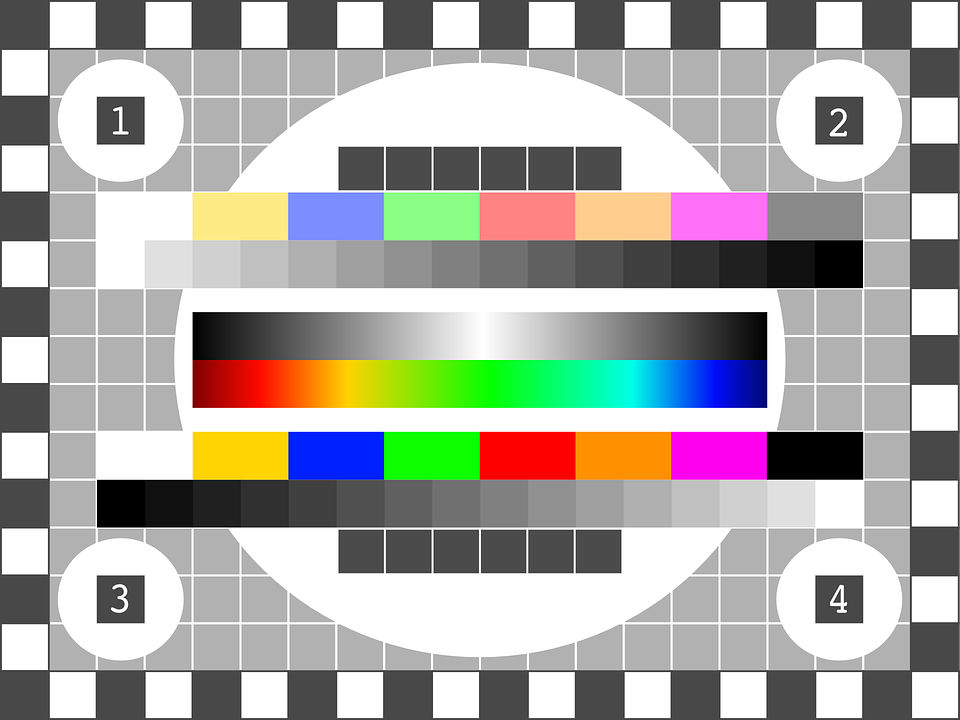
\includegraphics[width=1\textwidth]{figures/test}
\end{center}
\caption{Overordnet løsningsforslag. }
\label{fig:loesningsforslag}
\end{figure}


\section{Metode til løsning}\label{metode_loesningsforslag}

I de følgende afsnit vil hvert element som ses på figur \ref{fig:loesningsforslag} blive beskrevet og hvert element vil få funktionelle og fysiske krav, en accept test af disse samt en afgrænsning. Ud fra kravspecifikationer vil et samlet system blive designet ud fra hvert element. En priorteringsliste vil blive udarbejdet ud fra "vigtigheden" af elementerne i systemet og disse vil blive implementeret i denne rækkefølge. Herefter vil en test følge der tager udgangspunkt i det samlede system og accept test af hvert element af systemet. 

